\documentclass[11pt,letterpaper]{article}

% ==================================================
% PAQUETES
% ==================================================

\usepackage[utf8]{inputenc}
\usepackage[T1]{fontenc}
\usepackage[spanish]{babel}
\usepackage{amsmath,amssymb}
\usepackage{graphicx}
\usepackage{geometry}
\usepackage{array}
\usepackage{longtable}
\usepackage{booktabs}
\usepackage{float}
\usepackage{fancyvrb}
\usepackage{hyperref}
\usepackage{xcolor}

% ==================================================
% CONFIGURACION
% ==================================================

\geometry{margin=2.2cm}

\setlength{\parindent}{0pt}
\setlength{\parskip}{5pt}

\sloppy

\hypersetup{
    colorlinks=true,
    linkcolor=black,
    urlcolor=blue
}

% Configuracion de los archivos de texto
\fvset{
    fontsize=\scriptsize,
    frame=single,
    numbers=none
}

\begin{document}

% ==================================================
% PORTADA
% ==================================================

\begin{titlepage}
\centering

\vspace*{1.5cm}

{\Large Universidad Nacional Autónoma de México\par}

\vspace{0.5cm}

{\Large Facultad de Ciencias\par}

\vspace{2cm}

{\Large Laboratorio de Compiladores\par}

\vspace{1.5cm}

{\Huge\bfseries Práctica 5\par}

\vspace{0.5cm}

{\LARGE Parsers LR(0) y SLR(1)\par}

\vspace{2cm}

{\Large\bfseries Jesús Eliuth Martínez Mendoza\par}

\vfill

{\Large Octubre de 2026\par}

\end{titlepage}

% ==================================================
% 1. GRAMATICA Y TOKENS
% ==================================================

\section*{1. Gramática numerada y tokens}

Para esta práctica desarrollamos un analizador sintáctico
SLR(1) en lenguaje C, utilizando una gramática que permite
reconocer secuencias de comandos sencillos relacionados
con operaciones sobre archivos.

También se incorporaron expresiones aritméticas con sumas
y paréntesis para representar estructuras que requieren
un análisis sintáctico más elaborado.

La gramática está formada por 20 producciones originales
y una producción aumentada.

\subsection*{1.1. Producciones}

\begin{longtable}{|c|l|}
\hline
\textbf{Núm.} & \textbf{Producción} \\ \hline
0 & $S' \rightarrow Programa$ \\ \hline
1 & $Programa \rightarrow Lista$ \\ \hline
2 & $Lista \rightarrow Lista\ Comando$ \\ \hline
3 & $Lista \rightarrow Comando$ \\ \hline
4 & $Comando \rightarrow crear\ Archivo\ ;$ \\ \hline
5 & $Comando \rightarrow borrar\ Archivo\ ;$ \\ \hline
6 & $Comando \rightarrow copiar\ Archivo\ Archivo\ ;$ \\ \hline
7 & $Comando \rightarrow mover\ Archivo\ Archivo\ ;$ \\ \hline
8 & $Comando \rightarrow mostrar\ Archivo\ ;$ \\ \hline
9 & $Comando \rightarrow buscar\ Archivo\ ;$ \\ \hline
10 & $Comando \rightarrow renombrar\ Archivo\ Archivo\ ;$ \\ \hline
11 & $Comando \rightarrow listar\ ;$ \\ \hline
12 & $Comando \rightarrow ejecutar\ Accion\ ;$ \\ \hline
13 & $Accion \rightarrow Accion + Elemento$ \\ \hline
14 & $Accion \rightarrow Elemento$ \\ \hline
15 & $Elemento \rightarrow id$ \\ \hline
16 & $Elemento \rightarrow num$ \\ \hline
17 & $Elemento \rightarrow (\ Accion\ )$ \\ \hline
18 & $Archivo \rightarrow id$ \\ \hline
19 & $Archivo \rightarrow ruta$ \\ \hline
20 & $Archivo \rightarrow nombre$ \\ \hline
\end{longtable}

\subsection*{1.2. Símbolos terminales}

Los símbolos terminales reconocidos por la gramática son:

\begin{center}
\begin{tabular}{|l|p{10cm}|}
\hline
\textbf{Categoría} & \textbf{Terminales} \\ \hline
Comandos &
crear, borrar, copiar, mover, mostrar, buscar,
renombrar, listar, ejecutar \\ \hline
Archivos & id, ruta, nombre \\ \hline
Expresiones & num, +, (, ) \\ \hline
Separador & ; \\ \hline
Fin de entrada & \$ \\ \hline
\end{tabular}
\end{center}

El símbolo \$ se utiliza para indicar que la entrada
ha terminado.

\subsection*{1.3. Símbolos no terminales}

Los símbolos no terminales son:

\[
\{
Programa, Lista, Comando,
Accion, Elemento, Archivo
\}
\]

El símbolo inicial es $Programa$.

Para construir el analizador se utiliza la producción
aumentada:

\[
S' \rightarrow Programa
\]

\subsection*{1.4. Características de la gramática}

La gramática permite reconocer uno o varios comandos
consecutivos.

Cada comando debe respetar su estructura y finalizar
con punto y coma.

Por ejemplo, la producción:

\[
Lista \rightarrow Lista\ Comando
\]

permite construir secuencias de comandos.

Por otra parte:

\[
Accion \rightarrow Accion + Elemento
\]

introduce recursividad por la izquierda y permite
representar expresiones con varias sumas.

La producción:

\[
Elemento \rightarrow (\ Accion\ )
\]

permite utilizar paréntesis dentro de las expresiones.

% ==================================================
% 2. DESARROLLO MATEMATICO
% ==================================================

\section*{2. Desarrollo matemático del analizador}

Para construir el analizador SLR(1), primero calculamos
los conjuntos FIRST y FOLLOW.

Después obtuvimos la colección canónica de elementos
LR(0), identificamos las transiciones del autómata y
construimos las matrices ACTION y GOTO.

Finalmente analizamos los conflictos presentes en LR(0)
y comprobamos cómo se resuelven utilizando SLR(1).

% ==================================================
% FIRST
% ==================================================

\subsection*{2.1. Conjuntos FIRST}

El conjunto FIRST de un símbolo no terminal contiene
los terminales con los que puede comenzar una cadena
derivada de dicho símbolo.

Los conjuntos obtenidos fueron:

\begin{center}
\begin{tabular}{|l|p{10cm}|}
\hline
\textbf{No terminal} & \textbf{FIRST} \\ \hline
Programa &
crear, borrar, copiar, mover, mostrar,
buscar, renombrar, listar, ejecutar \\ \hline
Lista &
crear, borrar, copiar, mover, mostrar,
buscar, renombrar, listar, ejecutar \\ \hline
Comando &
crear, borrar, copiar, mover, mostrar,
buscar, renombrar, listar, ejecutar \\ \hline
Accion & id, num, ( \\ \hline
Elemento & id, num, ( \\ \hline
Archivo & id, ruta, nombre \\ \hline
\end{tabular}
\end{center}

\subsubsection*{Justificación}

La producción:

\[
Programa \rightarrow Lista
\]

indica que FIRST(Programa) depende de FIRST(Lista).

A su vez:

\[
Lista \rightarrow Lista\ Comando
\]

\[
Lista \rightarrow Comando
\]

permite concluir que cualquier lista comienza
con alguno de los terminales que inician un comando.

Por lo tanto:

\[
FIRST(Programa)=FIRST(Lista)=FIRST(Comando)
\]

Para el símbolo Archivo tenemos:

\[
Archivo \rightarrow id
\]

\[
Archivo \rightarrow ruta
\]

\[
Archivo \rightarrow nombre
\]

De donde obtenemos:

\[
FIRST(Archivo)=\{id,ruta,nombre\}
\]

Finalmente:

\[
Accion \rightarrow Elemento
\]

y las producciones de Elemento permiten comenzar
con un identificador, un número o un paréntesis.

Por ello:

\[
FIRST(Accion)=FIRST(Elemento)=\{id,num,(\}
\]

% ==================================================
% FOLLOW
% ==================================================

\subsection*{2.2. Conjuntos FOLLOW}

El conjunto FOLLOW de un símbolo no terminal contiene
los terminales que pueden aparecer inmediatamente
después de dicho símbolo en alguna derivación.

Los conjuntos obtenidos fueron:

\begin{center}
\begin{tabular}{|l|p{10cm}|}
\hline
\textbf{No terminal} & \textbf{FOLLOW} \\ \hline
Programa & \$ \\ \hline
Lista &
\$, crear, borrar, copiar, mover, mostrar,
buscar, renombrar, listar, ejecutar \\ \hline
Comando &
\$, crear, borrar, copiar, mover, mostrar,
buscar, renombrar, listar, ejecutar \\ \hline
Accion & +, ), ; \\ \hline
Elemento & +, ), ; \\ \hline
Archivo & id, ruta, nombre, ; \\ \hline
\end{tabular}
\end{center}

\subsubsection*{Justificación}

Como Programa es el símbolo inicial:

\[
FOLLOW(Programa)=\{\$\}
\]

En la producción:

\[
Lista \rightarrow Lista\ Comando
\]

después de Lista aparece Comando.

Por lo tanto:

\[
FIRST(Comando)\subseteq FOLLOW(Lista)
\]

Además, Lista puede terminar al final de la entrada,
por lo que \$ también pertenece a FOLLOW(Lista).

Como Comando aparece al final de las producciones
de Lista, hereda su conjunto FOLLOW.

Para Archivo, observamos que puede aparecer
seguido de otro Archivo o de un punto y coma.

De esta manera:

\[
FOLLOW(Archivo)=\{id,ruta,nombre,;\}
\]

Para las expresiones, la gramática permite que
Accion y Elemento aparezcan antes de un operador
de suma, un paréntesis de cierre o un punto y coma.

Por ello:

\[
FOLLOW(Accion)=FOLLOW(Elemento)=\{+,),;\}
\]

% ==================================================
% COLECCION CANONICA
% ==================================================

\subsection*{2.3. Colección canónica de elementos LR(0)}

Para obtener los estados del analizador comenzamos
con la producción aumentada:

\[
S' \rightarrow \cdot Programa
\]

Aplicamos la operación de cerradura, también
conocida como CLOSURE.

Esta operación incorpora las producciones de los
símbolos no terminales que aparecen inmediatamente
después del punto.

Formalmente, si un conjunto contiene:

\[
A \rightarrow \alpha \cdot B\beta
\]

se incorporan los elementos:

\[
B \rightarrow \cdot \gamma
\]

para cada producción de B.

Posteriormente aplicamos la operación GOTO para
desplazar el punto y obtener nuevos estados.

Como resultado, construimos una colección canónica
formada por 45 estados, numerados desde
$I_0$ hasta $I_{44}$.

A continuación se presentan todos los elementos
de la colección canónica:

\VerbatimInput{../docs/estados_lr0.txt}

% ==================================================
% TRANSICIONES
% ==================================================

\subsection*{2.4. Transiciones GOTO del autómata LR(0)}

La operación GOTO permite determinar el estado
al que se llega cuando se reconoce un símbolo
terminal o no terminal.

Formalmente:

\[
GOTO(I,X)=
CLOSURE\left(
\left\{
A\rightarrow\alpha X\cdot\beta
\mid
A\rightarrow\alpha\cdot X\beta\in I
\right\}
\right)
\]

Donde I representa un conjunto de elementos LR(0)
y X representa un símbolo de la gramática.

Aplicando esta operación obtuvimos 88 transiciones
entre los 45 estados.

Las transiciones son:

\VerbatimInput{../docs/transiciones_lr0.txt}

% ==================================================
% MATRICES
% ==================================================

\subsection*{2.5. Matrices ACTION y GOTO}

Una vez construida la colección canónica LR(0),
utilizamos sus estados y transiciones para
definir las matrices ACTION y GOTO.

La tabla ACTION indica qué operación debe realizar
el analizador al consultar un estado y el siguiente
token de entrada.

Las acciones posibles son:

\begin{itemize}
    \item \textbf{SHIFT:} desplaza un token y cambia de estado.
    \item \textbf{REDUCE:} aplica una producción de la gramática.
    \item \textbf{ACCEPT:} acepta la cadena de entrada.
    \item \textbf{ERROR:} indica que no existe una acción válida.
\end{itemize}

La tabla GOTO se consulta después de una reducción
para determinar el nuevo estado a partir del símbolo
no terminal producido.

En nuestra implementación utilizamos 45 estados,
18 terminales incluyendo el marcador \$,
y 6 símbolos no terminales.

Las matrices completas son:

\VerbatimInput{../docs/matrices_slr1.txt}

En estas matrices:

\begin{itemize}
    \item $s_j$ representa un desplazamiento al estado $j$.
    \item $r_k$ representa una reducción por la producción $k$.
    \item \texttt{acc} representa la aceptación.
    \item El símbolo \texttt{-} representa una entrada sin acción.
\end{itemize}

Las columnas de ACTION siguen este orden:

\begin{Verbatim}[fontsize=\scriptsize]
crear borrar copiar mover mostrar buscar renombrar listar
ejecutar id ruta nombre num + ( ) ; $
\end{Verbatim}

Las columnas de GOTO siguen este orden:

\begin{Verbatim}[fontsize=\scriptsize]
Programa Lista Comando Accion Elemento Archivo
\end{Verbatim}

% ==================================================
% CONFLICTOS
% ==================================================

\subsection*{2.6. Conflictos LR(0) y resolución SLR(1)}

Durante la construcción del analizador identificamos
un estado que presenta conflictos de tipo
desplazamiento/reducción cuando se utiliza LR(0).

Este conflicto aparece en el estado $I_2$.

Entre sus elementos se encuentran:

\[
Programa \rightarrow Lista\cdot
\]

\[
Lista \rightarrow Lista\cdot Comando
\]

El primer elemento indica que es posible realizar
una reducción mediante la producción:

\[
r_1:\ Programa \rightarrow Lista
\]

Sin embargo, el segundo elemento permite continuar
reconociendo otro comando.

Por lo tanto, en LR(0) existen dos acciones posibles
para los terminales que inician un comando:

\begin{itemize}
    \item Reducir mediante la producción 1.
    \item Desplazar el siguiente comando.
\end{itemize}

Los terminales involucrados son:

\[
\begin{gathered}
crear,\ borrar,\ copiar,\ mover,\ mostrar,\\
buscar,\ renombrar,\ listar,\ ejecutar
\end{gathered}
\]

Esto produce nueve celdas con conflicto
desplazamiento/reducción en el estado $I_2$.

\subsubsection*{Resolución mediante FOLLOW}

En SLR(1), una reducción:

\[
A\rightarrow\alpha\cdot
\]

solamente se coloca en las columnas de ACTION
correspondientes a los terminales de FOLLOW(A).

En nuestro caso:

\[
FOLLOW(Programa)=\{\$\}
\]

Por lo tanto, la reducción $r_1$ únicamente
se coloca en la columna \$.

Las nueve columnas correspondientes a los comandos
conservan sus acciones SHIFT.

Así obtenemos:

\[
ACTION[I_2,\$]=r_1
\]

y para cada terminal que inicia un comando:

\[
ACTION[I_2,a]=SHIFT
\]

De esta manera desaparecen los nueve conflictos
presentes en LR(0).

Es importante señalar que se trata de un solo
estado conflictivo, pero de nueve celdas
con conflicto.

La matriz SLR(1) resultante no presenta
conflictos de desplazamiento/reducción
ni de reducción/reducción.

% ==================================================
% 3. ARQUITECTURA
% ==================================================

\section*{3. Arquitectura del analizador}

El analizador se desarrolló en lenguaje C y se
organizó en diferentes módulos para separar
la lectura de tokens, el análisis sintáctico,
las tablas y la construcción del árbol.

\subsection*{3.1. Diagrama de arquitectura}

\begin{figure}[H]
    \centering
    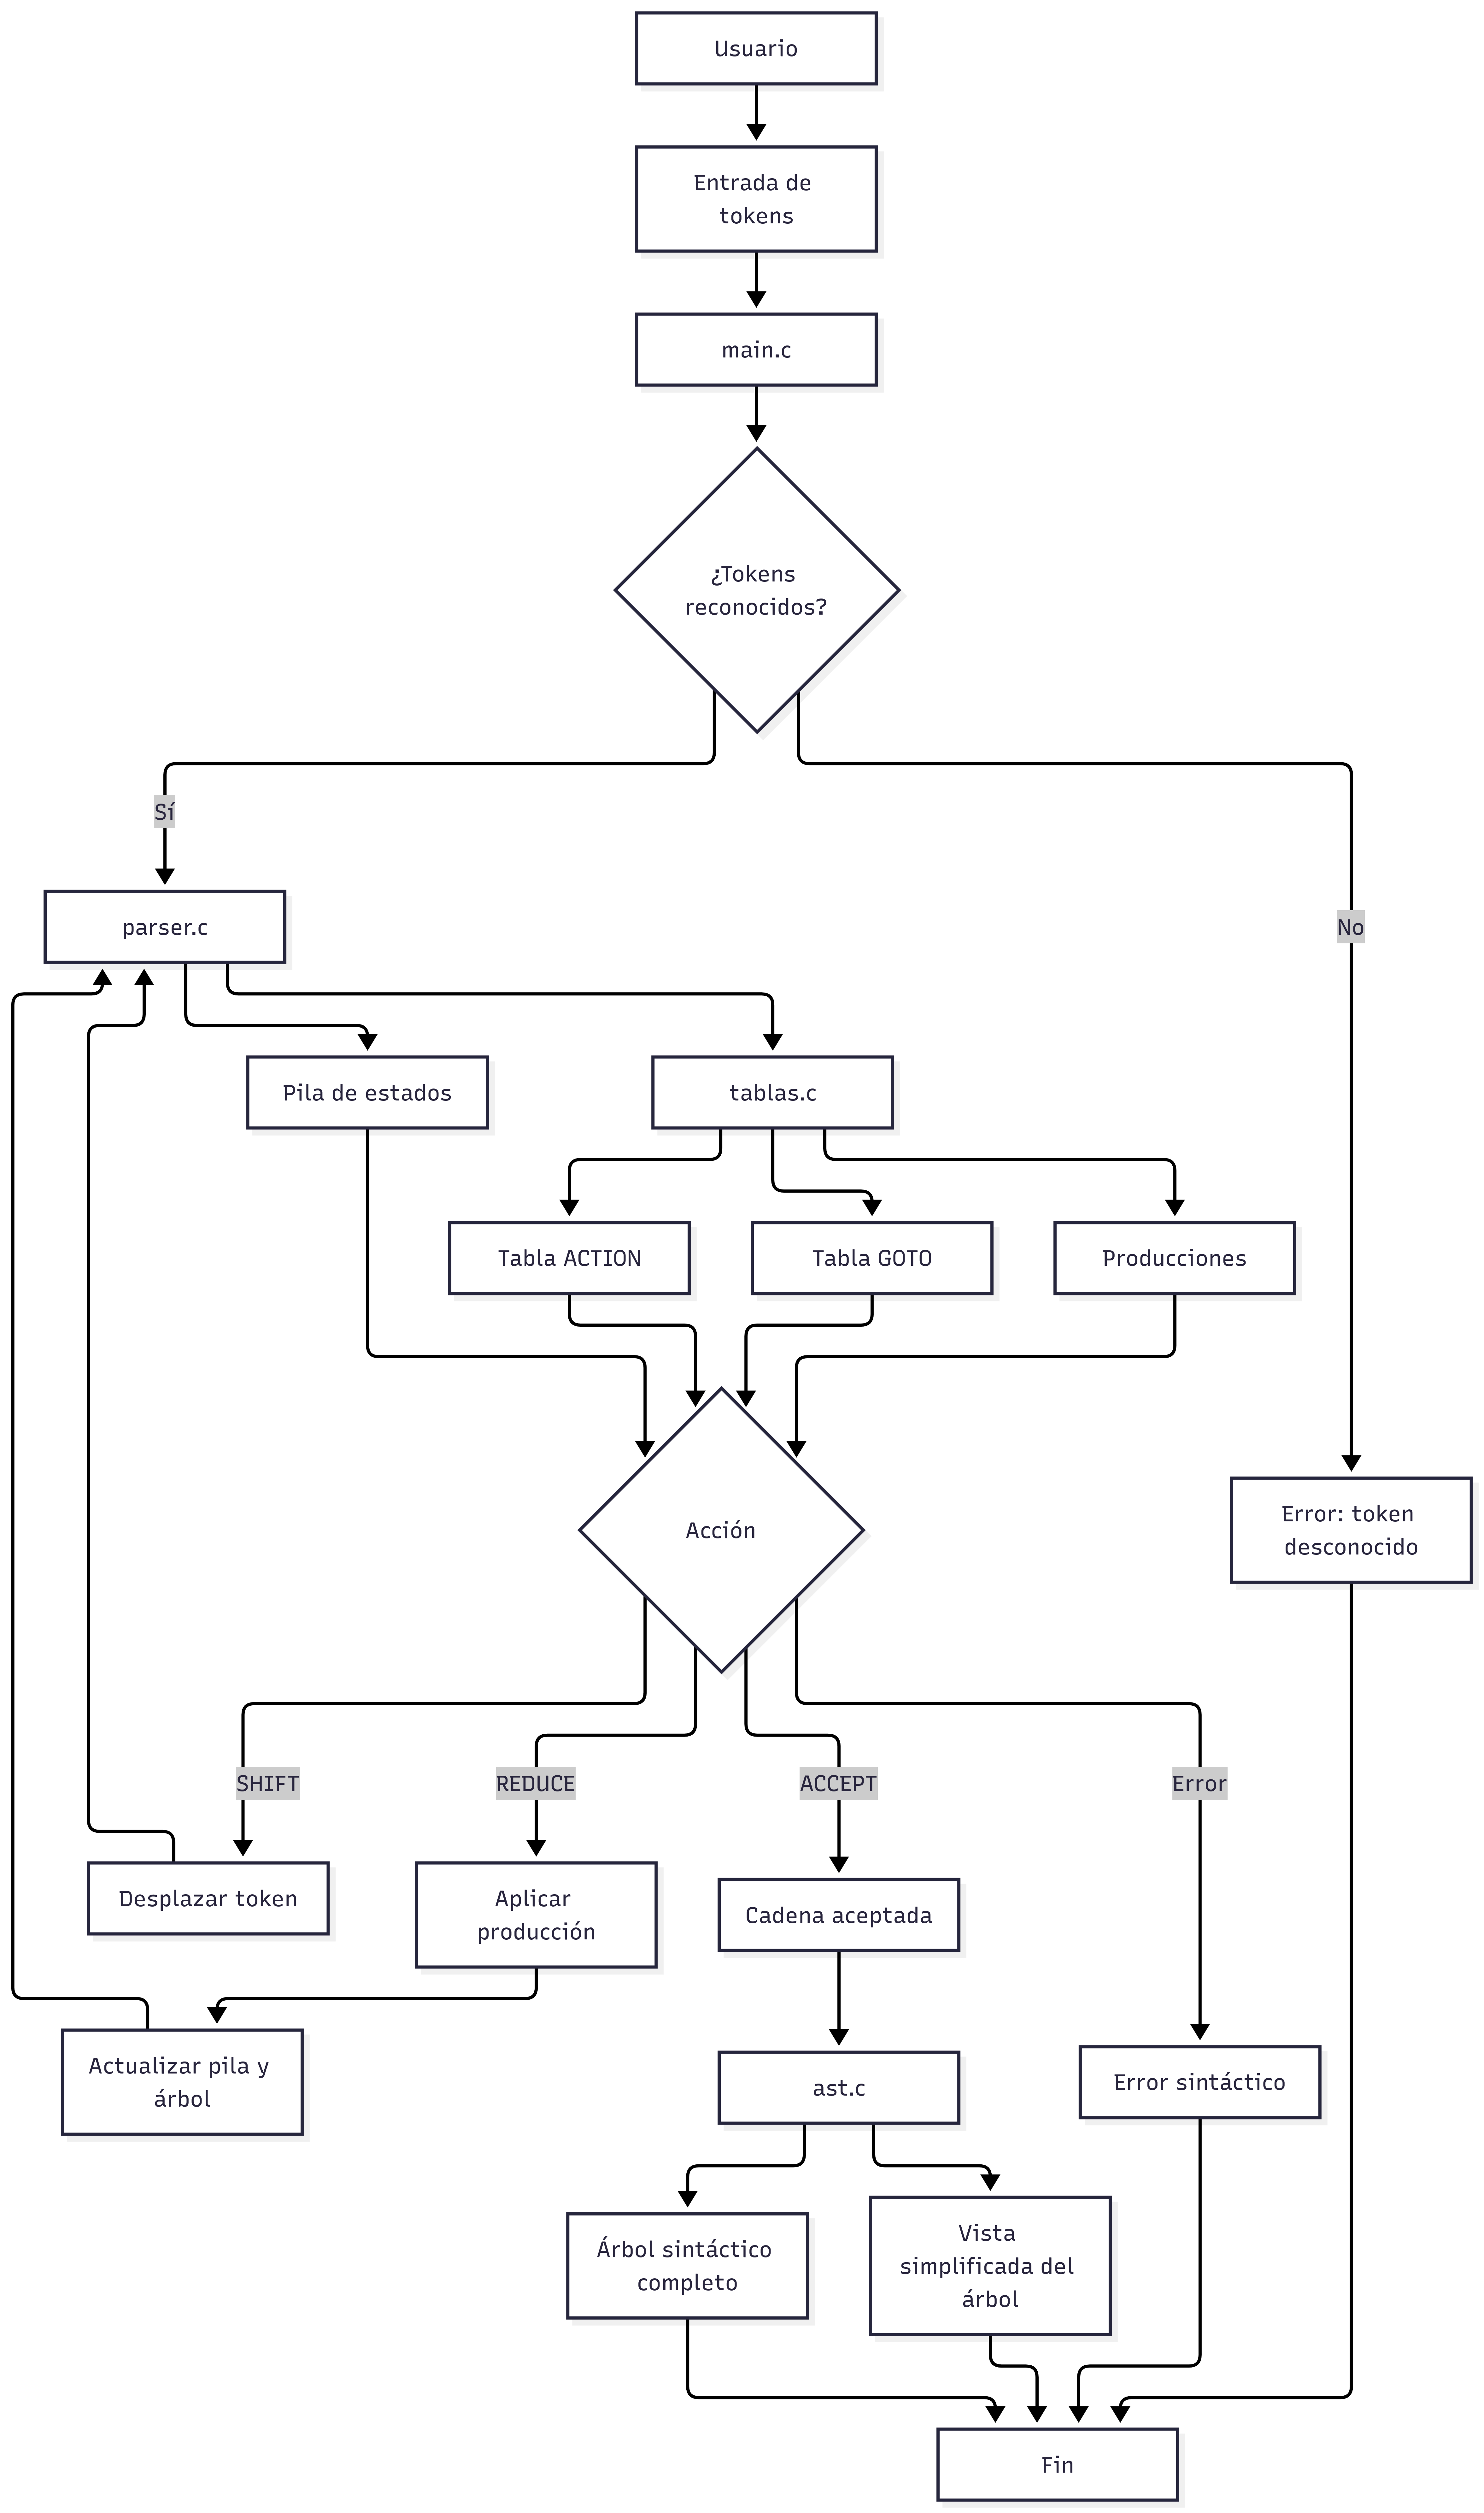
\includegraphics[
        width=0.95\textwidth,
        height=0.75\textheight,
        keepaspectratio
    ]{../docs/arquitectura_slr1.png}
    \caption{Arquitectura general del analizador SLR(1).}
\end{figure}

\subsection*{3.2. Componentes principales}

\textbf{main.c}

Es el punto de entrada del programa.
Recibe la secuencia de tokens proporcionada
por el usuario y prepara la entrada para
el análisis sintáctico.

\textbf{parser.c}

Contiene el funcionamiento principal del
analizador SLR(1).

Administra la pila de estados y símbolos,
consulta las tablas y ejecuta las operaciones
SHIFT, REDUCE y ACCEPT.

También identifica errores sintácticos.

\textbf{tablas.c}

Contiene las matrices ACTION y GOTO
definidas directamente en lenguaje C.

También almacena la información de las
producciones utilizadas durante las reducciones.

\textbf{ast.c}

Contiene las funciones utilizadas para construir,
mostrar y liberar los nodos del árbol sintáctico.

Además, permite presentar una versión simplificada
del árbol, eliminando elementos que no son necesarios
para representar la estructura principal.

\textbf{include/}

Contiene las declaraciones, estructuras y
constantes que comparten los diferentes módulos.

\subsection*{3.3. Funcionamiento del analizador}

El funcionamiento general es el siguiente:

\begin{enumerate}
    \item El usuario introduce una secuencia de tokens.
    \item El programa identifica los tokens de entrada.
    \item Se inicializa la pila con el estado 0.
    \item Se consulta ACTION utilizando el estado actual
          y el siguiente token.
    \item Si la acción es SHIFT, se desplaza el token
          y se actualiza la pila.
    \item Si la acción es REDUCE, se aplica la producción
          correspondiente y se consulta GOTO.
    \item Si aparece ACCEPT, la cadena se acepta
          y se muestran los árboles sintácticos.
    \item Si no existe una acción válida,
          se informa que la cadena es incorrecta.
\end{enumerate}

El programa también muestra las operaciones
realizadas durante el análisis, lo que permite
observar cómo cambia la pila en cada paso.

% ==================================================
% 4. PRUEBAS
% ==================================================

\section*{4. Pruebas del analizador}

Para comprobar el funcionamiento del analizador
realizamos diez pruebas automáticas.

Cinco pruebas utilizan cadenas válidas y las
otras cinco contienen errores.

Las pruebas permiten verificar el reconocimiento
de comandos, las secuencias de instrucciones,
las expresiones y la detección de errores.

\small

\begin{longtable}{|c|p{4.4cm}|p{1.6cm}|p{6cm}|}
\hline
\textbf{Prueba} &
\textbf{Entrada} &
\textbf{Resultado} &
\textbf{Justificación} \\ \hline
\endfirsthead

\hline
\textbf{Prueba} &
\textbf{Entrada} &
\textbf{Resultado} &
\textbf{Justificación} \\ \hline
\endhead

01 &
\texttt{crear id ;} &
Válida &
Cumple la estructura del comando crear y termina
correctamente con punto y coma. \\ \hline

02 &
\texttt{crear id ; borrar ruta ; listar ;} &
Válida &
Contiene tres comandos consecutivos que cumplen
con las producciones de la gramática. \\ \hline

03 &
\texttt{copiar id ruta ; mover nombre id ;} &
Válida &
Los comandos copiar y mover contienen los dos
argumentos de tipo Archivo que necesitan. \\ \hline

04 &
\texttt{ejecutar id + num + id ;} &
Válida &
La gramática permite expresiones con varias
sumas mediante recursividad por la izquierda. \\ \hline

05 &
\texttt{ejecutar ( id + num ) + id ;} &
Válida &
Los paréntesis y los operadores están colocados
correctamente. \\ \hline

06 &
\texttt{crear id} &
Inválida &
Falta el punto y coma que debe aparecer
al finalizar el comando. \\ \hline

07 &
\texttt{copiar id ;} &
Inválida &
El comando copiar requiere dos argumentos
de tipo Archivo y solamente se proporcionó uno. \\ \hline

08 &
\texttt{ejecutar id + ;} &
Inválida &
Después del operador de suma debe aparecer
otro Elemento. \\ \hline

09 &
\texttt{ejecutar ( id + num ;} &
Inválida &
Falta el paréntesis de cierre de la expresión. \\ \hline

10 &
\texttt{eliminar id ;} &
Inválida &
La palabra eliminar no pertenece a los
terminales reconocidos por la gramática. \\ \hline

\end{longtable}

\normalsize

\subsection*{4.1. Resultados obtenidos}

Las diez pruebas produjeron los resultados esperados.

Las cinco cadenas válidas fueron aceptadas.

De las cinco cadenas inválidas, cuatro fueron
rechazadas por errores sintácticos y una por
contener un token desconocido.

Los resultados completos de cada prueba se
guardaron en el directorio:

\begin{center}
\texttt{pruebas/resultados/}
\end{center}

Esto permitió comprobar que el analizador
reconoce las estructuras definidas en la
gramática y detecta los errores de las
entradas utilizadas durante las pruebas.

% ==================================================
% 5. REPOSITORIO
% ==================================================

\section*{5. Repositorio público}

El código fuente del analizador, las tablas
SLR(1), la documentación y los casos de prueba
se organizaron dentro del proyecto.

El repositorio público permite consultar
los archivos utilizados durante el desarrollo
y reproducir las pruebas realizadas.

\textbf{Enlace al repositorio:}

\begin{center}
\texttt{PENDIENTE: agregar enlace público de GitHub}
\end{center}

% ==================================================
% NOTA SOBRE ACTIVIDAD PENDIENTE
% ==================================================

% El ejercicio adicional de auditoria con IA
% se incorporara cuando se complete y revise.
% No debe entregarse el reporte como definitivo
% mientras esa actividad siga pendiente.

\end{document}
